\documentclass[10pt]{article}
\usepackage{sdss2020}
\usepackage{url}
\usepackage{latexsym}
\usepackage{amsmath, amsthm, amsfonts}
\usepackage{algorithm, algorithmic}  
\usepackage{graphicx}
\usepackage{booktabs}
\usepackage{multirow}
\usepackage{float}
\usepackage[spanish]{babel}
\usepackage{hyperref}
\usepackage[utf8]{inputenc}

\title{
    DIFRACCIÓN DE ELECTRONES EN UNA RED POLICRISTALINA\\
    Universidad del Valle \\
    Departamento de Física, experimentación en Física III
}

\author{
    Nicolás Aguilera García \\
    {\tt 2021273030} \\
    \And
    Andrés Felipe Valencia Fonseca \\
    {\tt 202125166} \\
    \And 
    Kevin Giraldo Hincapie\\
    {\tt 202024236} \\
}

\date{}




\begin{document}
    \maketitle

    \begin{abstract}
        En esta práctica se analiza el comportamiento de un sistema de difracción de electrones en una red policristalina, con el objetivo de evidenciar y verificar la ecuación dada por B’roglie para la longitud de onda de los electrones. De los resultados, al medir los diámetros de anillos de difracción se obtuvo que la longitud de onda de los electrones experimentales se acercan a los valores teóricos, lo cual confirma la ecuación de B’roglie.
        Por otro lado, se determinó de la constante de Plank mediante un proceso de regresión lineal, de donde se obtuvieron dos valores, uno de los cuales se descarta por contar con un error relativo del $150.65\%$, y como valor aceptable esta que la constante de Plank es $6.071 \pm 0.03 \times 10^{-34} J.s$.


        {\bf Keywords: } Difracción de electrones, longitud de onda, Constante de Plank.
    \end{abstract}


    \section{Análisis de datos}
    Partiendo de los resultados obtenidos durante la práctica de laboratorio, se utilizó los valores experimentales de $D_1$ y $D_2$ para calcular la longitud de onda $\lambda_1$ y $\lambda_2$ respectivamente, los cuales se muestran en las tablas \ref{tab:datosD1} y \ref{tab:datosD2}.

    El cálculo de las longitudes experimentales se realizó con la siguiente ecuación, la cual se dedujo de a partir de las relaciones de las distancias inter planares del grafito:
    \begin{equation}
        \lambda = d\frac{D}{2L}
    \end{equation}
    Donde $d$ es la distancia reticular inter planar, $D$ es el diámetro del anillo y $L$ es la distancia entre el grafito y la pantalla.

    Estos valores de longitud de onda se compararon con los valores teóricos de la longitud de onda de los electrones en el grafito, los cuales se muestran en las tablas \ref{tab:datosD1} y \ref{tab:datosD2} respectivamente. El valor de la longitud de onda teórica se obtuvo de la siguiente ecuación:
    \begin{equation}
        \lambda = \frac{h}{\sqrt{2em_eV}}
    \end{equation}

    \begin{table}[H]
        \centering
        \resizebox{3.3in}{!} {
            \begin{tabular}{cccc}
                \hline
                \multicolumn{1}{l|}{U (kV)} & \multicolumn{1}{l|}{$D_1 \pm \delta D_1$ (cm)}    & \multicolumn{1}{l|}{$\lambda_1 \pm \delta \lambda_1 $ (pm)}   & $\lambda_{1,teorica}$ (pm) \\ \hline
                $2.9$                       & $3.91 \pm 0.10$                                           & $30.85 \pm 1.64$                                                       & $ 22.80 $                      \\
                $3.5$                       & $3.24 \pm 0.10$                                           & $25.56 \pm 1.62$                                                       & $ 20.75 $                      \\
                $4.0$                       & $2.64 \pm 0.10$                                           & $20.79 \pm 1.61$                                                       & $ 19.41 $                      \\
                $4.5$                       & $2.56 \pm 0.10$                                           & $20.16 \pm 1.61$                                                       & $ 18.30 $                      \\ \hline
            \end{tabular}
        }
        \label{tab:datosD1}
        \caption{Medición del diametro $D_1$ y su correspondiente longitud de onda $\lambda_1$ determinada experimentalmente y su valor teórico.}
    \end{table}

    \begin{table}[H]
        \centering
        \resizebox{3.3in}{!} {
            \begin{tabular}{cccc}
                \hline
                \multicolumn{1}{l|}{U (kV)} & \multicolumn{1}{l|}{$D_2 \pm \delta D_2$ (cm)}    & \multicolumn{1}{l|}{$\lambda_2 \pm \delta \lambda_2 $ (pm)}   & $\lambda_{2,teorica}$ (pm) \\ \hline
                $2.9$                       & $5.31 \pm 0.10$                                           & $24.19 \pm 0.98$                                                       & $ 22.80 $                      \\
                $3.5$                       & $4.83 \pm 0.10$                                           & $22.00 \pm 0.97$                                                       & $ 20.75 $                      \\
                $4.0$                       & $4.67 \pm 0.10$                                           & $21.26 \pm 0.96$                                                       & $ 19.41 $                      \\
                $4.5$                       & $4.37 \pm 0.10$                                           & $19.88 \pm 0.96$                                                       & $ 18.30 $                      \\ \hline
            \end{tabular}
        }
        \label{tab:datosD2}
        \caption{Medición del diametro $D_2$ y su correspondiente longitud de onda $\lambda_2$ determinada experimentalmente y su valor teórico.}
    \end{table}

    Finalmente, se determinó dos valores de la constante de Planck, $h_1$ y $h_2$, los cuales se obtuvieron al partir de la siguiente relación:
    \begin{equation}
        \begin{split}
            D &= k\frac{1}{\sqrt{U}} \\
            k &= \frac{2Lh}{d\sqrt{2em_e}}
        \end{split}
    \end{equation}

    De donde se puede determinar el valor de $k$ como la pendiente de la recta con intercepto nulo que se obtiene al graficar $D$ en función de $\frac{1}{\sqrt{U}}$. Esta regresión lineal se muestra en la figura \ref{fig:regresion}.

    \begin{figure}[h]
        \centering
        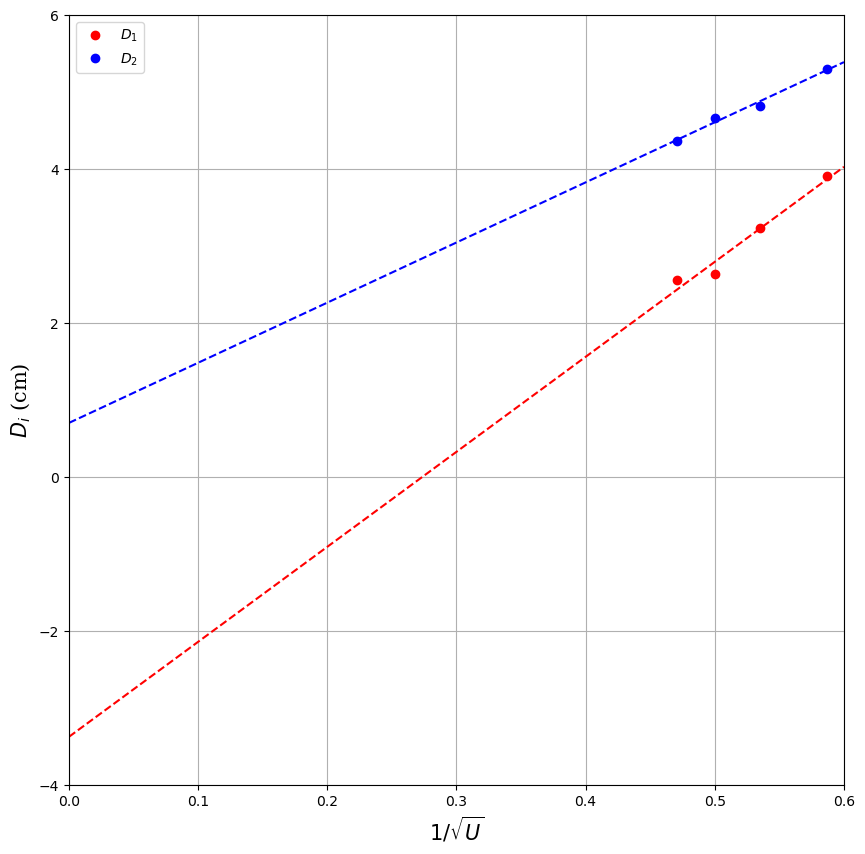
\includegraphics[width=3.3in]{img/regresion.png}
        \caption{Regresión lineal de la constante de $D_i$ en función de $\frac{1}{\sqrt{U}}$.}
        \label{fig:regresion}
    \end{figure}

    Las ecuaciones que se obtienen al realizar la regresión lineal son las siguientes:

    \begin{itemize}
        \item $D_1 = -3.368 + 12.337 \frac{1}{\sqrt{U}}$
        \item $D_2 = 0.709 + 7.809 \frac{1}{\sqrt{U}}$
    \end{itemize}

    De donde se obtienen los valores de la constante de Planck como:

    \begin{itemize}
        \item $h_1 = 1.661 \pm 0.03 \times 10^{-33} J.s$
        \item $h_2 = 6.071 \pm 0.03 \times 10^{-34} J.s$
    \end{itemize}

    Se evidencia que el valor obtenido mediante $D_2$ es más cercano al valor real de la constante de Planck con un error relativo de $8.38\%$ mientras que el valor obtenido mediante $D_1$ tiene un error relativo de $150.65\%$.

    \section{Conclusiones}
        Con los resultados de la primera parte del laboratorio se pudo verificar la relación dada por la ecuación de B’roglie que relaciona la longitud de onda de una partícula con su momento lineal. Y aunque los valores de la longitud de onda obtenidos no son exactamente iguales a los valores teóricos, estos se encuentran dentro de la incertidumbre experimental.

        Ahora para la determinación de la constante de Planck, es evidente la diferencia entre los valores obtenidos de $h$ mediante $D_1$ y $D_2$, llegando a tener diferencia de un orden de magnitud, este error fue previsible al ver los resultados de la regresión lineal, en donde ambas regresiones contaban con interceptó no nulo (la obtenida médiate $D_2$ es más cercana a $0$) lo cual era condición necesaria para poder determinar el valor de $h$ mediante la ecuación utilizada.

        Sin embargo, aun con la diferencia en los resultados de $h$ el valor $h_2$ puede ser tomado como aceptable, ya que el error relativo es de $8.38\%$, valor que puede ser atribuido a la incertidumbre experimental.
\end{document}
